% Section 1: Introduction

\section{Introduction}

Optimal transport is widely used in the field of computer science, especially in areas as computer graphics, computer vision, medical image processing and deep learning. As the product of the intersection of multiple disciplines, it contains problems from probability, analysis, and optimization. The main objective of the research is to establish a geometric tool for efficient comparison of probability distributions, that is, the modeling of probability distributions by geometric methods and the measurement of the distance between probability distributions is a bridge connecting geometry and probability.

Take the problem given by the French mathematician Monge more than 200 years ago as an example: When two sand plates are given (each sand plate can represent a probability distribution), a sand plate can be transmitted in many ways (Transport or Reshape) to another sandbox. Based on the local cost of transmitting a single sand particle, each transport method corresponds to a global cost. The purpose of optimal transport is to find the transport solution with the lowest overall cost, so as to further establish the geometric toolset for probability distribution.

The optimal transport problem has a long and rich research history, which can be traced back to the eighteenth-century Monge mentioned above. The Russian mathematician Kantorovich gave a more practical form of relaxation in the 1940s and was further promoted in the 1990s because of a series of important mathematical theoretical achievements, including important work of French mathematician Brenier. It is particularly important that many Fields Prize winners have made important contributions in the study of optimal transport theory, such as the French mathematician Cédric Villani (The Fields Award 2010), Italian Mathematics Alessio Figalli (The Fields Award 2018), and has many important monographs \cite{book1, book2, book3, book4}. In terms of application, optimal transport has been widely used in the field of computer science, especially in computer graphics, computer vision, medical image processing, and deep learning.

In order to introduce the optimal transmission problem more concisely, we only consider the optimal transmission problem for discrete probability vectors (histograms). First, a probability vector or histogram refers to a vector $a \in \Sigma_m$ belongs to a set of probability simplex, that is,

\begin{equation}
  \Sigma_{m}:=\left\{\mathbf{a} \in \mathbb{R}_{+}^{m}: \sum_{i=1}^{m} \mathbf{a}_{i}=1\right\}
\end{equation}

Due to the computational difficulty of the optimal transport problem proposed by Monge and the limitation of this model, the Kantorovich relaxed optimal transport model has drawn attention in academia. By removing the limitation of fully deterministic transport (the quantity of the same point cannot be decomposed), Kantorovich gives a concise and effective optimal transport model. Transport is achieved through the Couplings matrix $P_+^{n \times m}$, where the set of coupling matrices is defined as

\begin{equation}
  \mathbf{U}(\mathbf{a}, \mathbf{b}) \stackrel{\text { def. }}{=}\left\{\mathbf{P} \in \mathbb{R}_{+}^{m \times n}: \mathbf{P} \mathbf{1}_{n}=\mathbf{a} \quad \text { and } \quad \mathbf{P}^{\mathrm{T}} \mathbf{1}_{m}=\mathbf{b}\right\}
\end{equation}

$\mathbf{a} \in \Sigma_m$ and $\mathbf{b} \in \Sigma_n$ are both probability vectors or histograms. The coupling matrix set is bounded and consists of $m + n$ equality constraints, which can be regarded as a convex polyhedron. 

Kantorovich optimal transmission problem can be defined as

\begin{equation}
  \mathcal{L}_{\mathbf{C}}(\mathbf{a}, \mathbf{b}):=\min _{\mathbf{P} \in \mathbf{U}(\mathbf{a}, \mathbf{b})}\langle\mathbf{C}, \mathbf{P}\rangle:=\sum_{i, j} \mathbf{C}_{i j} \mathbf{P}_{i j}
\end{equation}

Where $C \in \mathbb{R}^{n \times m}$ represents the cost matrix and $C_{ij}$ represents the cost required to transfer from $i$ to $j$. The Kantorovich optimal transport problem is a linear programming problem, and the problem does not necessarily have a unique solution. The importance of the optimal transport problem is not only in itself, it provides a way to meaningfully characterize the distance between probability vectors or histograms.

\vspace{5ex}
\begin{figure}[htbp]
  \centering
  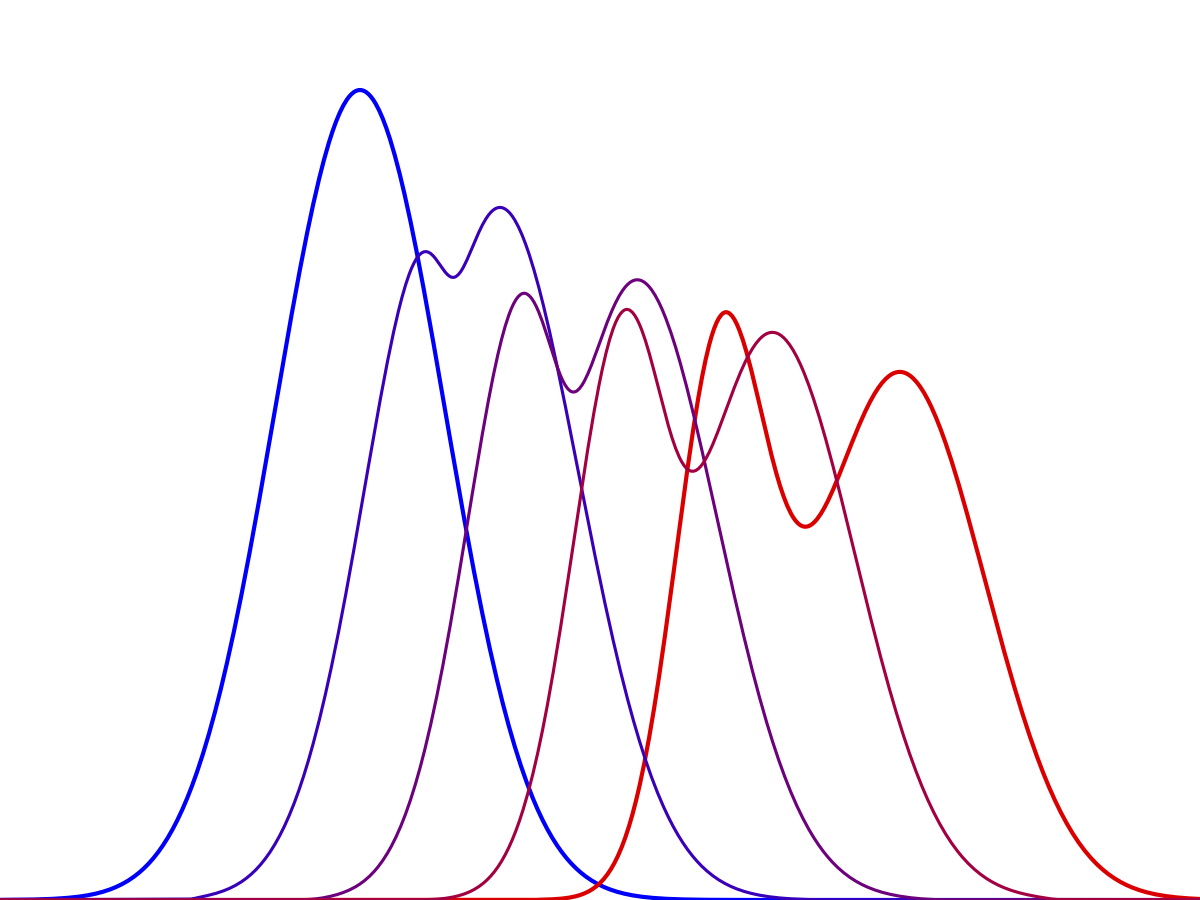
\includegraphics[width=0.8\linewidth]{img/ot}
  \label{fig:ot}
  \caption{Illustration of Optimal Transport Interpolation}
\end{figure}